In this chapter, we will introduce the \emph{\index{discrete Fourier
    transform}{discrete Fourier transform}} (DFT). We will also briefly
discuss the \emph{\index{fast Fourier transform}{fast Fourier transform}} (FFT) algorithm,
which is a very efficient numerical algorithm that can be used to evaluate a DFT.

The importance of the DFT and the FFT algorithm cannot be sufficiently
stressed. Its use is ubiquitous in modern signal processing. Much of
the technology that you use in your everyday life is dependent on this
algorithm. Whenever you are watching a video or displaying an image on
your computer screen, listening to digital music, or using a wireless
internet connection, you are with a high likelihood using technology
that relies on the DFT implemented using the FFT algorithm.
\begin{marginfigure}
  \hrulefill \newline

  \noindent \textbf{Fourier Series}\newline

  \begin{equation*}
    x(t)=\sum_{k=-\infty}^{\infty} c_k e^{i \frac{2\pi k}{T} t}
  \end{equation*}
  \begin{equation*}
    c_k=\frac{1}{T}\int_{T} x(t) e^{-i \frac{2\pi k}{T}  t} dt
  \end{equation*}
  Periodic in time: \newline $x(t+T)=x(t)$\newline

  \noindent \hrulefill
  \newline
  \noindent \textbf{Fourier Transform}
  \newline
  \begin{equation*}
    x(t) = \frac{1}{2\pi}\int_{-\infty}^{\infty} \hat{x}(\omega) e^{i\omega t} d\omega
  \end{equation*}
  \begin{equation*}
    \hat{x}(\omega) = \int_{-\infty}^{\infty} x(t) e^{-i\omega t} dt
  \end{equation*}
  \newline
  \noindent \hrulefill
  \newline

  \noindent \textbf{Discrete-time Fourier Transform}
  \newline
  \begin{equation*}
    x[n] = \frac{1}{2\pi} \int_{2\pi} \hat{x}(\hat{\omega}) e^{i\hat{\omega} n} d\hat{\omega}
  \end{equation*}
  \begin{equation*}
    \hat{x}(\hat{\omega}) = \sum_{n=-\infty}^{\infty} x[n] e^{-i\hat{\omega} n}
  \end{equation*}
  Periodic in frequency:\newline $\hat{x}(\hat{\omega}) = \hat{x}(\hat{\omega}+2\pi)$
  \newline
  \noindent \hrulefill

  \noindent \textbf{Discrete Fourier Transform}
  \newline
  \begin{equation*}
    x[n] = \frac{1}{N}\sum_{k=0}^{N-1}\hat{x}[k] e^{i\frac{2\pi}{N}kn}
  \end{equation*}
  \begin{equation*}
    \hat{x}[k] = \sum_{n=0}^{N-1}x[n] e^{-i\frac{2\pi}{N}kn}
  \end{equation*} \newline
  Periodic in time and frequency: \newline$x[n+ N]=x[n]$\newline $\hat{x}[k+ N]=\hat{x}[k]$
  \newline
  \noindent \hrulefill

  \caption{A summary of all the frequency domain representations of a
    signal covered so far in this course.
    The discrete Fourier transform will be covered in this chapter.}
  \label{fig:summary_fourier}
\end{marginfigure}

The DFT is widely used in practical signal processing applications,
which are impossible to exhaustively list here. For example, the DFT
can be used:
\begin{itemize}
  \item to approximate a Fourier transform
  \item to approximate a discrete-time Fourier transform,
  \item for spectral analysis of signals,
  \item to efficiently implement a convolution of two signals,
  \item in spectral  compression algorithms (e.g., the MP3 and JPEG sound and image formats),
  \item to interpolate and re-sample signals,
  \item for filtering signals,
  \item for modulation and demodulation of radio signals in telecommunications, or
  \item to solve differential equations (e.g., Poisson's equation).
\end{itemize}
This is just a small fraction of the applications of the DFT and the FFT algorithm.

\section{Derivation of the discrete Fourier transform}

The DFT is a frequency domain representation for \index{periodic
  discrete-time signals}{periodic
  discrete-time signals} $x[n]=x[n+N]$. Because the time domain signal is
discrete-time and periodic, it follows that the frequency domain
representation is also a periodic discretized signal
$\hat{x}[k]=\hat{x}[k+N]$. Let's see why.

\begin{marginfigure}
  \begin{center}
    \begin{tikzpicture}
      \begin{axis}[
          width=7cm,height=5cm,ymin=-2.5,xmin=-4,ymax=5,xmax=6,
          xtick={-3,-1,1,2,3,4,5,6},
          xticklabels={$-3T_s$,$-T_s$,$T_s$,$2T_s$,$3T_s$,$4T_s$,$5T_s$},
          yticklabels={,,,},
          ylabel={$x_d(t)$},
          xlabel=$t$, axis lines = center]
        \addplot+[dirac] plot coordinates { ( -3,3 ) ( -2,2 ) ( -1,1) ( 0,3 ) ( 1,2 ) ( 2,1) ( 3,3 ) ( 4,2 ) ( 5,1 )  };
        \node at (axis cs:1,2.2) [above, blue, font={\footnotesize}]{$x[1]$};
        \node at (axis cs:2,1.2) [above, blue, font={\footnotesize}]{$x[2]$};
        \node at (axis cs:-3,3.2) [above, blue, font={\footnotesize}]{$x[0]$};
        \node at (axis cs:-2,2.2) [above, blue, font={\footnotesize}]{$x[1]$};
        \node at (axis cs:-1,1.2) [above, blue, font={\footnotesize}]{$x[2]$};
        \node at (axis cs:3,3.2) [above, blue, font={\footnotesize}]{$x[0]$};
        \node at (axis cs:4,2.2) [above, blue, font={\footnotesize}]{$x[1]$};
        \node at (axis cs:5,1.2) [above, blue, font={\footnotesize}]{$x[2]$};

        \node at (axis cs:4.5,3.7) [above, red, font={\footnotesize}]{$T_s$};
        \addplot [dimen,red]plot coordinates {(4.0,3.7) (5.0,3.7)};

        \addplot [dimen,red]plot coordinates {(0.0,-1.5) (3.0,-1.5)};
        \node at (axis cs:1.5,-1.5) [below, red, font={\footnotesize}]{$N T_s$};
      \end{axis}
    \end{tikzpicture}
  \end{center}
  \caption{A continuous-time representation of a periodic discretized signal. In this example, the period of the
  discrete-time signal is $N=3$, which means that $x[n]=x[n+3]$. The sample-spacing is $T_s$, which implies that
  the period of this signal in continuous-time is $N T_s$.}
  \label{fig:example_periodic_xd}
\end{marginfigure}

Consider the following continuous-time signal, which has a
period of $N T_s$:
\begin{equation}
  x_d(t) = \sum_{p=-\infty}^{\infty} \sum_{n=0}^{N-1} x[n] \delta(t - n T_s - p N T_s ) \,\,.
  \label{eq:dtft_time_per0}
\end{equation}
This is a continuous-time representation of a periodic discrete-time
signal $x[n]$ with period $N$, sampled with sample-spacing $T_s =
  1/f_s$. Here $f_s$ is sample-rate. The index $p$ is used to create
infinitely many copies of the signal with time offsets of
$pNT_s$. I've made an example plot of this type of signal in
Figure \ref{fig:example_periodic_xd}. In the example $N=3$, which
means that $x_d(t)=x_d(t+3T_s)$.

Because this signal is periodic, we can use the Fourier series to
represent this signal as a sum of complex sinusoidal signals:
\begin{equation}
  x_d(t) = \sum_{k=-\infty}^{\infty} c_k e^{i\frac{2\pi}{NT_s}kt}  = \sum_{k=-\infty}^{\infty} c_k e^{i \omega_k t} \,\,.
\end{equation}
We can use the Fourier series analysis formula to determine the coefficients $c_k$:
\begin{align}
  c_k & = \frac{1}{N T_s} \int_{0}^{N T_S} x_d(t) e^{-i\frac{2\pi}{N T_s}kt}dt                                                                                     \\
      & = \frac{1}{N T_s} \int_{0}^{N T_S} \left(\sum_{p=-\infty}^{\infty} \sum_{n=0}^{N-1} x[n] \delta(t - n T_s - p N T_s ) \right) e^{-i\frac{2\pi}{N T_s}kt}dt \\
      & = \frac{1}{N T_s} \sum_{n=0}^{N-1} x[n] \int_{0}^{N T_S} \delta(t - n T_s)  e^{-i\frac{2\pi}{N T_s}kt}dt                                                   \\
      & =  \frac{1}{N T_s} \sum_{n=0}^{N-1} x[n]  e^{-i\frac{2\pi}{N T_s}k n T_s}                                                                                  \\
      & =  \frac{1}{N T_s} \sum_{n=0}^{N-1} x[n] e^{-i\frac{2\pi}{N}kn  }                                                                                          \\
      & =  \frac{1}{N T_s} \hat{x}[k] \,\, _.
\end{align}
The last term
\begin{equation}
  \hat{x}[k] = \sum_{n=0}^{N-1} x[n] e^{-i\frac{2\pi}{N}kn  } \,\,,
  \label{eq:dtft_fs_0}
\end{equation}
is the discrete Fourier transform. It is up to a constant $1/NT_s$, the
Fourier series coefficient that corresponds to the spectral component
with angular frequency
\begin{equation}
  \boxed{
    \omega_k = \frac{2\pi}{N T_s}k
  } \,\,,
\end{equation}
in a Fourier series representation of $x_d(t)$. This equation can
be used to relate the $k$th spectral component to continuous-time
angular frequency.

\begin{marginfigure}
  \begin{center}
    \begin{tikzpicture}
      \begin{axis}[
          width=7cm,
          height=5cm,
          ymin=-2.5,
          xmin=-4,
          ymax=5,
          xmax=6,
          xtick={-3,-1,1,3,5},
          xticklabels={$-3\Delta \omega$,$-\Delta \omega$,$\Delta \omega$,$3\Delta \omega$,$5\Delta \omega$},
          yticklabels={,,,},
          ymajorticks=false,
          ylabel={$\frac{N T_s}{2\pi} \hat{x}_d(\omega)$},
          xlabel=$\omega$, axis lines = center]
        \addplot+[dirac] plot coordinates { ( -3,3 ) ( -2,2 ) ( -1,1) ( 0,3 ) ( 1,2 ) ( 2,1) ( 3,3 ) ( 4,2 ) ( 5,1 )  };
        \node at (axis cs:1,2.2) [above, blue, font={\footnotesize}]{$\hat{x}[1]$};
        \node at (axis cs:2,1.2) [above, blue, font={\footnotesize}]{$\hat{x}[2]$};
        \node at (axis cs:-3,3.2) [above, blue, font={\footnotesize}]{$\hat{x}[0]$};
        \node at (axis cs:-2,2.2) [above, blue, font={\footnotesize}]{$\hat{x}[1]$};
        \node at (axis cs:-1,1.2) [above, blue, font={\footnotesize}]{$\hat{x}[2]$};
        \node at (axis cs:3,3.2) [above, blue, font={\footnotesize}]{$\hat{x}[0]$};
        \node at (axis cs:4,2.2) [above, blue, font={\footnotesize}]{$\hat{x}[1]$};
        \node at (axis cs:5,1.2) [above, blue, font={\footnotesize}]{$\hat{x}[2]$};

        \node at (axis cs:4.5,3.7) [above, red, font={\footnotesize}]{$\Delta \omega$};
        \addplot [dimen,red]plot coordinates {(4.0,3.7) (5.0,3.7)};

        \addplot [dimen,red]plot coordinates {(0.0,-1.5) (3.0,-1.5)};
        \node at (axis cs:1.5,-1.5) [below, red, font={\footnotesize}]{$\omega_s$};
      \end{axis}
    \end{tikzpicture}
  \end{center}
  \caption{The spectral representation of a periodic discretized signal
    $\hat{x}_d(\omega)=\hat{x}_d(\omega+\omega_s)$, multiplied by $N T_s/2\pi$.
    In this example, $N=3$. The frequency step between unit impulses is $\Delta \omega = \frac{\omega_s}{N}$.}
  \label{fig:example_periodic_fd}
\end{marginfigure}

By inspecting Equation \ref{eq:dtft_fs_0}, it is easy to see that
$\hat{x}[k]=\hat{x}[k+N]$. This means that the Fourier series
coefficients repeat every $N$ points.

We can Fourier transform $x_d(t)$ to obtain the frequency domain
representation:
\begin{align}
  \hat{x}_d(\omega) & = \int_{-\infty}^{\infty} x_d(t) e^{-i\omega t}d\omega                                                                          \\
                    & = \int_{-\infty}^{\infty} \left(\sum_{k=-\infty}^{\infty} c_k e^{i\omega_k t}\right) e^{-i\omega t} d\omega                     \\
                    & = \sum_{k=-\infty}^{\infty} c_k \int_{-\infty}^{\infty}  e^{i(\omega_k-\omega) t} d\omega                                       \\
                    & = \frac{2\pi}{N T_s}\sum_{k=-\infty}^{\infty} \hat{x}[k] \delta\left(\omega_k-\omega\right)                                     \\
                    & = \frac{2\pi}{N T_s}\sum_{p=-\infty}^{\infty} \sum_{k=0}^{N-1} \hat{x}[k] \delta\left(\omega_k-\omega - p \omega_s\right) \,\,.
  \label{eq:dtft_freq_0}
\end{align}
In the last line, I have emphasized the fact that $\hat{x}[n]$ is a
periodic signal with period $N$. Periodicity of $\hat{x}[k]$ implies
that $\hat{x}_d(\omega)$ is also periodic $\hat{x}_d(\omega)
  = \hat{x}_d(\omega+\omega_s)$ with period $\omega_s = 2\pi f_s$.

An example plot of $\hat{x}_d(\omega)$ scaled by $N T_s/2\pi$ is shown
in Figure \ref{fig:example_periodic_fd}. In this example $N=3$, which
means that $\hat{x}[k]=\hat{x}[k+3]$.

By comparing equations \ref{eq:dtft_freq_0}
and \ref{eq:dtft_time_per0}, we can see that both are similar
continuous-time representations of a periodic discrete signal. One is
a periodic discrete-time signal $x[n]=x[n+N]$ and the other is a
periodic discrete-frequency signal $\hat{x}[k]=\hat{x}[k+N]$. The
period of both signals is $N$.


\newpage
\section{Discrete Fourier Transform}

The \index{discrete Fourier transform}{discrete Fourier transform} (DFT) is defined as:
\begin{equation}
  \boxed{
    \hat{x}[k] = \mathcal{F}_D\{x[n]\} =\sum_{n=0}^{N-1} x[n] e^{-i\frac{2\pi}{N} nk}
  } \,\,.
  \label{eq:dft_forward_eq}
\end{equation}
It is used to obtain the complex amplitude of the spectral components
for normalized angular frequencies\sidenote{
  With Python, you can use the \texttt{numpy.fft.fftfreq} command
  to calculate the continuous-time frequency $f_k$ corresponding to each frequency component $\hat{x}[k]$.
}:
\begin{equation}
  \boxed{
    \hat{\omega}_k = \frac{2\pi}{N}k
  } \,\,.
\end{equation}
We use the notation $\hat{x}[k]$ to denote the discrete nature of the
spectral representation.

The inverse operation, i.e., the operation that converts the frequency
domain representation $\hat{x}[k]$ into a time domain representation
$x[n]$ is the \index{inverse discrete Fourier transform}{inverse discrete Fourier transform} (IDFT), which is
defined as:
\begin{equation}
  \boxed{
  x[n] = \mathcal{F}_D^{-1}\{\hat{x}[k]\} = \frac{1}{N}\sum_{k=0}^{N-1} \hat{x}[k] e^{i\frac{2\pi}{N} nk}
  } \,\,.
\end{equation}
The term $1/N$ is a required normalization constant, which is by
convention typically attached to the inverse transform.

We'll prove the reversibility of the transform
$x[n]=\mathcal{F}_D^{-1}\{\mathcal{F}_D\{x[n]\}\}$ by expressing the DFT
using orthogonal basis vectors $\bm{\psi}_k$.

\subsection{Orthogonal basis vectors}

\usetikzlibrary{calc,angles,quotes}
\usetikzlibrary{quotes,angles}
\begin{marginfigure}
  \begin{center}
    \begin{tikzpicture}
      \coordinate (v1) at (0,0);
      \coordinate (v2) at (0,2);
      \coordinate (v3) at (2,0);

      \coordinate (b0) at (0,0);
      \coordinate (b1) at (0.2,0);
      \coordinate (b2) at (0.2,0.2);
      \coordinate (b3) at (0,0.2);
      \draw[->] (v1) -- node[left] {$\bm{\psi}_{k}$} (v2);
      \draw[->] (v1) -- node[below] {$\bm{\psi}_{\ell}$} (v3);

      % draw line and angle
      \draw [very thin] (b0) -- (b1) -- (b2) -- (b3)-- (b0);
    \end{tikzpicture}
  \end{center}
  \caption{The discrete Fourier transform \index{basis vectors}{basis vectors} are
  orthogonal $\bm{\psi}_{k} \perp \bm{\psi}_{\ell}$ for all $\ell \ne k$.
  This implies that $\bm{\psi}_k^{H}\bm{\psi}_{\ell} = 0$ when $\ell \ne k$.}
\end{marginfigure}

Let's first define a phase constant $\phi=e^{-i\frac{2\pi}{N}}\in\mathbb{C}$, which implies that
\begin{equation}
  \phi^{kn} = e^{-i\frac{2\pi}{N}kn} \,\,,
\end{equation}
we can use this to define basis vectors $\bm{\psi}_k \in \mathbb{C}^{N \times 1}$ as:
\begin{equation}
  \bm{\psi}_k  = \begin{bmatrix}
    \phi^{k\cdot0} & \phi^{k\cdot1} & \phi^{k\cdot2} & \cdots & \phi^{k\cdot(N-1)}
  \end{bmatrix}^T \,\,.
\end{equation}
All $N$ unique basis vectors orthogonal with one another, i.e., the inner product is:
\begin{align}
  \bm{\psi}_k^H \bm{\psi}_{\ell} & = \sum_{n=0}^{N-1} e^{i\frac{2\pi}{N}(k-\ell)n} \\
                                 & = N \delta_{k,\ell} \,\,.
\end{align}
I've used the \index{Kronecker delta}{Kronecker delta} $\delta_{k,\ell}$ here, which is defined as:
\begin{equation}
  \delta_{k,\ell}=\left\{
  \begin{array}{cc}
    1 & k=\ell     \\
    0 & k \ne \ell
  \end{array}\right.  \,\, _.
\end{equation}
The proof is divided into two cases. First, when $k=\ell$:
\begin{align}
  \bm{\psi}_k^H \bm{\psi}_{k} = \sum_{n=0}^{N-1}  e^{i\frac{2\pi}{N}(k-k)n} = \sum_{n=0}^{N-1} e^{0} = N \,\,.
\end{align}
and when $k\ne \ell$
\begin{align}
  \bm{\psi}_k^H  \bm{\psi}_{\ell} = \sum_{n=0}^{N-1} e^{i\frac{2\pi}{N}n(k-\ell)} = S \,\,.
\end{align}
We can use a \index{geometric series}{geometric series} to solve for $S$:
\begin{align*}
  S          & = \alpha^0 + \cdots + \alpha^{N-1}    \\
  \alpha S   & = \alpha^1 + \cdots + \alpha^{N}      \\
  S-\alpha S & = 1 - \alpha^N                        \\
  S          & = \frac{1-\alpha^N}{1-\alpha} \,\, _.
\end{align*}
With $\alpha = e^{i\frac{2\pi}{N}(k-\ell)}$, we obtain:
\begin{align}
  \sum_{n=0}^{N-1} e^{i\frac{2\pi}{N}(k-\ell)n} & = \frac{1-1}{1-e^{i\frac{2\pi}{N}(k-\ell)}} = 0 \,\,.
\end{align}
This proves that the \index{discrete Fourier transform basis vectors}{discrete Fourier transform basis vectors}
$\bm{\psi}_k$ are orthogonal.

\subsection{Reversibility of the transform}

Let's define a vector $\bm{\hat{x}}$ that contains the $N$ spectral
components $\hat{x}[k]$ obtained using a DFT:
\begin{equation}
  \bm{\hat{x}}=\begin{bmatrix}
    \hat{x}[0] & \hat{x}[1] & \hat{x}[2] & \cdots \hat{x}[N-1]
  \end{bmatrix}^T \in \mathbb{C}^{N\times 1} \,\,.
\end{equation}
We also define a vector  $\bm{x}$, which contains the $N$ elements of the periodic signal $x[n]$:
\begin{equation}
  \bm{x}=\begin{bmatrix}
    x[0] & x[1] & x[2] & \cdots & x[N-1]
  \end{bmatrix}^T \in \mathbb{C}^{N\times 1} \,\,.
\end{equation}
Finally, let's define a matrix $\bm{F}\in\mathbb{C}^{N\times N}$ by
stacking the $N$ basis vectors $\bm{\psi}_k$:
\begin{align*}
  \bm{F} & = \begin{bmatrix}
               \bm{\psi}_0^T \\
               \bm{\psi}_1^T \\
               \bm{\psi}_2^T \\
               \vdots        \\
               \bm{\psi}_{N-1}^T
             \end{bmatrix} = \begin{bmatrix}
                               \phi^{0\cdot0}     & \phi^{0 \cdot 1}     & \phi^{0 \cdot 2}     & \cdots & \phi^{0 \cdot (N-1)}     \\
                               \phi^{1\cdot0}     & \phi^{1 \cdot 1}     & \phi^{1 \cdot 2}     & \cdots & \phi^{1 \cdot (N-1)}     \\
                               \phi^{2\cdot0}     & \phi^{2 \cdot 1}     & \phi^{2 \cdot 2}     & \cdots & \phi^{2 \cdot (N-1)}     \\
                               \vdots             &                      &                      & \ddots & \vdots                   \\
                               \phi^{(N-1)\cdot0} & \phi^{(N-1) \cdot 1} & \phi^{(N-1) \cdot 2} & \cdots & \phi^{(N-1) \cdot (N-1)} \\
                             \end{bmatrix} \,\,.
\end{align*}
Using this matrix, we can express the forward and reverse discrete Fourier transforms as matrix-vector products:
\begin{align}
  x[n] = \mathcal{F}_D^{-1}\{\hat{x}[k]\} & \xleftrightarrow{\mathcal{F}_D} \hat{x}[k] = \mathcal{F}_D\{x[n]\} \\
  \bm{x}=\frac{1}{N}\bm{F}^H\bm{\hat{x}}  & \xleftrightarrow{\mathcal{F}_D} \bm{\hat{x}}=\bm{F} \bm{x} \,\,.
\end{align}
We can now prove \index{reversibility}{reversibility}. A combination of a forward and 
reverse transform $x[n]=\mathcal{F}_D^{-1}\{\mathcal{F}_D\{x[n]\}\}$ is equivalent to:
\begin{equation}
  \bm{x} = \frac{1}{N}\bm{F}^H \bm{F} x \,\,.
\end{equation}
We can see that $\bm{F}^H \bm{F} = N\bm{I}$ is an identity matrix
multiplied with $N$:
\begin{align}
  \bm{F}^H \bm{F} & = \begin{bmatrix}
                        \bm{\psi}_0^H \bm{\psi}_0     & \bm{\psi}_0^H \bm{\psi}_1     & \bm{\psi}_0^H \bm{\psi}_2     & \cdots & \bm{\psi}_0^H \bm{\psi}_{N-1}     \\
                        \bm{\psi}_1^H \bm{\psi}_0     & \bm{\psi}_1^H \bm{\psi}_1     & \bm{\psi}_1^H \bm{\psi}_2     & \cdots & \bm{\psi}_1^H \bm{\psi}_{N-1}     \\
                        \bm{\psi}_2^H \bm{\psi}_0     & \bm{\psi}_2^H \bm{\psi}_1     & \bm{\psi}_2^H \bm{\psi}_2     & \cdots & \bm{\psi}_2^H \bm{\psi}_{N-1}     \\
                        \vdots                        &                               &                               & \ddots & \vdots                            \\
                        \bm{\psi}_{N-1}^H \bm{\psi}_0 & \bm{\psi}_{N-1}^H \bm{\psi}_1 & \bm{\psi}_{N-1}^H \bm{\psi}_2 & \cdots & \bm{\psi}_{N-1}^H \bm{\psi}_{N-1} \\
                      \end{bmatrix}=N\bm{I} \,\,.
\end{align}
This means that a combination of a forward and inverse transform results in the original 
discrete-time signal $\bm{x}$:
\begin{align}
  \bm{x} & = \frac{1}{N}\bm{F}^H \bm{F} \bm{x} \\
         & = \bm{x} \qed \,\,.
\end{align}
This proves the reversibility of the transform.

\section{Example: Periodic unit impulse}

Let us consider a periodic discrete-time signal
$\{x[n]\}_{n=0}^{N-1}=\{1,0,0,0\}$ of length $N=4$. This signal is
periodic, so $x[n+N]=x[n]$. The signal is shown in Figure \ref{fig:simple_per_4_imp}.
\begin{marginfigure}
  \begin{center}
    \begin{tikzpicture}
      \begin{axis}[
          width=7cm,
          height=6cm,
          ymin=0,
          xmin=-4,
          ymax=1.5,
          xmax=6,
          xtick={-3,-2,-1,0,1,2,3,4,5,6},
          ytick={0,1,2,3},
          ylabel={$x[n]$},
          xlabel={$n$}, axis lines = center]
        \addplot+[ycomb,color=black] plot coordinates { (0,1) (1,0) (2,0) (3,0)};
        \addplot+[ycomb,color=black] plot coordinates {(-4,1) (-3,0) (-2,0) (-1,0)  (4,1) (5,0) (6,0)};
      \end{axis}
    \end{tikzpicture}
    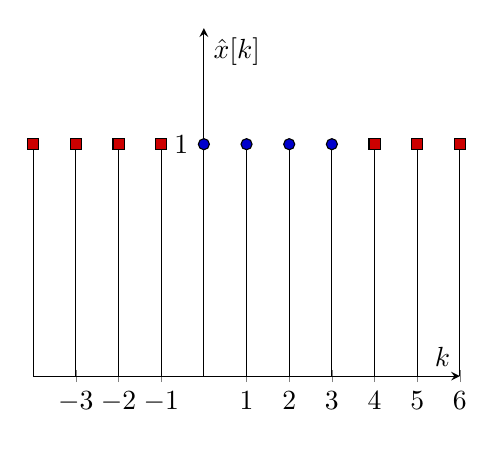
\begin{tikzpicture}
      \begin{axis}[
          width=7cm,
          height=6cm,
          ymin=0,
          xmin=-4,
          ymax=1.5,
          xmax=6,
          xtick={-3,-2,-1,0,1,2,3,4,5,6},
          ytick={0,1,2,3},
          ylabel={$\hat{x}[k]$},
          xlabel={$k$}, axis lines = center]
        \addplot+[ycomb,color=black] plot coordinates {(0,1) (1,1) (2,1) (3,1) };
        \addplot+[ycomb,color=black] plot coordinates {(-4,1) (-3,1) (-2,1) (-1,1)  (4,1) (5,1) (6,1)};
      \end{axis}
    \end{tikzpicture}
  \end{center}
  \caption{A periodic unit impulse in time domain results in a constant valued frequency domain representation.}
  \label{fig:simple_per_4_imp}
\end{marginfigure}

The DFT of this signal is:
\begin{align}
  \hat{x}[k] & = \sum_{n=0}^{3} x[n] e^{-i\frac{2\pi}{4}kn} \\
             & = 1 \,\,.
\end{align}
The spectrum $\hat{x}[k]$ is plotted in the bottom half of Figure \ref{fig:simple_per_4_imp}.
If we now take the inverse DFT of signal $\hat{x}[k]$, we get:
\begin{align}
  x[n] & = \frac{1}{4}\sum_{k=0}^{3} e^{i\frac{2\pi}{4}kn} \,\,.
\end{align}
For different values of $n$, we get:
\begin{align*}
  x[0] & = \frac{1}{4}(e^{i\frac{2\pi}{4}0\cdot 0} + e^{i\frac{2\pi}{4}1\cdot 0} + e^{i\frac{2\pi}{4}2\cdot 0} + e^{i\frac{2\pi}{4}3\cdot 0})=\frac{1}{4}(1 + 1 + 1 + 1) = 1,   \\
  x[1] & = \frac{1}{4}(e^{i\frac{2\pi}{4}0\cdot 1} + e^{i\frac{2\pi}{4}1\cdot 1} + e^{i\frac{2\pi}{4}2\cdot 1} + e^{i\frac{2\pi}{4}3\cdot 1}) = \frac{1}{4}(1 + i - 1 - i) = 0, \\
  x[2] & = \frac{1}{4}(e^{i\frac{2\pi}{4}0\cdot 2} + e^{i\frac{2\pi}{4}1\cdot 2} + e^{i\frac{2\pi}{4}2\cdot 2} + e^{i\frac{2\pi}{4}3\cdot 2}) = \frac{1}{4}(1 -1  + 1  -1) = 0, \\
  x[3] & = \frac{1}{4}(e^{i\frac{2\pi}{4}0\cdot 3} + e^{i\frac{2\pi}{4}1\cdot 3} + e^{i\frac{2\pi}{4}2\cdot 3} + e^{i\frac{2\pi}{4}3\cdot 3}) = \frac{1}{4}(1 - i - 1 + i) = 0.
\end{align*}
Which is the original signal $x[n]$.

% =============== NOT USED ===============
\if 0
  \section{Example: $\hat{x}[k] = N\delta[k]$}

  Let us consider a conversion of the example just shown before, where
  $\{\hat{x}[k]\}_{k=0}^{N-1}=\{4,0,0,0\}$. The discrete Fourier
  transform has length $N=4$. This corresponds to a signal with non-zero
  spectral components only at DC (zero-frequency). The spectrum
  $\hat{x}[k]$ is plotted below:
  \begin{marginfigure}
    \begin{center}
      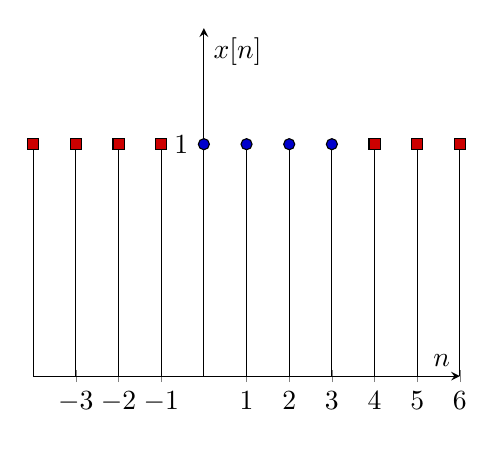
\begin{tikzpicture}
        \begin{axis}[width=7cm,height=6cm,ymin=0,xmin=-4,ymax=1.5,xmax=6,
            xtick={-3,-2,-1,0,1,2,3,4,5,6},
            ytick={0,1,2,3},
            ylabel={$x[n]$},
            xlabel={$n$}, axis lines = center]
          \addplot+[ycomb,color=black] plot coordinates { (0,1) (1,1) (2,1) (3,1)};
          \addplot+[ycomb,color=black] plot coordinates {(-4,1) (-3,1) (-2,1) (-1,1)  (4,1) (5,1) (6,1)};
        \end{axis}
      \end{tikzpicture}

      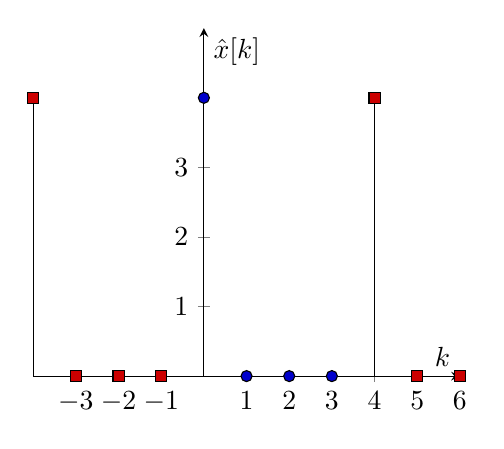
\begin{tikzpicture}
        \begin{axis}[width=7cm,height=6cm,ymin=0,xmin=-4,ymax=5,xmax=6,
            xtick={-3,-2,-1,0,1,2,3,4,5,6},
            ytick={0,1,2,3},
            ylabel={$\hat{x}[k]$},
            xlabel={$k$}, axis lines = center]
          \addplot+[ycomb,color=black] plot coordinates {(0,4) (1,0) (2,0) (3,0) };
          \addplot+[ycomb,color=black] plot coordinates {(-4,4) (-3,0) (-2,0) (-1,0)  (4,4) (5,0) (6,0)};
        \end{axis}
      \end{tikzpicture}

    \end{center}
    \caption{Example DFT.}
  \end{marginfigure}

  The IDFT of $\hat{x}[k]$ is:
  \begin{align}
    x[n] & = \frac{1}{4}\sum_{k=0}^{3}\hat{x}[k] e^{i\frac{2\pi}{4}kn} \\
         & = 1 \,\,.
  \end{align}
  This corresponds to a constant signal $\{x[n]\}_{n=0}^{3}=\{1,1,1,1\}$, which is shown below:

\fi

% =============== END ===============



\section{Relationship to the discrete-time Fourier transform}

The DTFT of a discrete-time signal is:
\begin{equation}
  \hat{x}(\hat{\omega}) = \sum_{n=-\infty}^{\infty} x[n] e^{-i\hat{\omega}n} \,\,.
\end{equation}
This is not a DFT, as $\hat{x}(\hat{\omega})$ is a continuous function
of $\hat{\omega}$, whereas $\hat{x}[k]$ is discrete in frequency.

For a finite-length signal $x[n] = 0$ when $n>N-1$ and $x[n] = 0$ when
$n<0$, the discrete-time Fourier transform is:
\begin{equation}
  \hat{x}(\hat{\omega}) = \sum_{n=0}^{N-1} x[n] e^{-i\hat{\omega}n} \,\,.
\end{equation}
Recall now the definition of the DFT:
\begin{align}
  \hat{x}[k] & = \sum_{n=0}^{N-1} x[n] e^{-ik\frac{2\pi}{N}n} \\
             & = \hat{x}(\hat{\omega}_k) \,\,.
\end{align}
This means that the DFT is the DTFT evaluated at discrete points:
\begin{equation}
  \boxed{
    \hat{\omega}_k=\frac{2\pi}{N}k
  } \,\,.
\end{equation}
The DFT can be seen as a special case of the DTFT. Note that nothing
about periodicity of signal $x[n]$ was assumed. We just assumed that
it was finite in length.

\section{Zero-padded DFT}

This immediately suggests a procedure for evaluating a DTFT
$\hat{x}(\hat{\omega})$ on $M$ evenly spaced frequencies
$\{0,\frac{2\pi}{M},\frac{4\pi}{M},\frac{6\pi}{M},\cdots,(M-1)\frac{2\pi}{M}\}$ using a DFT, where
$M>N$ is an integer larger than $N$, the length of the finite length
discrete-time signal $x[n]$.

We can do this with a \index{zero-padded DFT}{zero-padded DFT}. Zero padding means that we
define a zero-padded signal $x_{\mathrm{zp}}[n]$ of length $M$, which
has values
\begin{equation}
  x_{\mathrm{zp}}[n]=\left\{ \begin{array}{cc}
    x[n] & 0 \le n < N \\
    0    & N \le n < M
  \end{array}\right. \,\,.
\end{equation}
We then perform an $M$-point DFT:
\begin{equation}
  \boxed{
  \hat{x}_{\mathrm{zp}}[k] = \hat{x}(\hat{\omega}_k) = \sum_{n=0}^{M-1}x_{\mathrm{zp}}[n]e^{-i\frac{2\pi}{M}kn}
  } \,\,.
\end{equation}
This means that we can evaluate numerically the DTFT of a finite
length signal at $M$ evenly spaced points along the frequency axis. We
can select $M$ freely, to allow for arbitrary spacing of frequencies
at which the DTFT is evaluated.

\subsection{Example: Zero-padded DTFT estimate using DFT}

The Python code in Listing \ref{lst:dtft_estimate} demonstrates how to
estimate the DTFT of a signal using a DFT. In this example, we are
estimating the DTFT of the running average filter,
\begin{equation}
  y[n]=\frac{1}{L}\sum_{k=0}^{L-1}x[n-k] \,\,,
\end{equation}
which is an FIR filter with filter coefficients:
\begin{equation}
  h[n] = \frac{1}{L}\sum_{k=0}^{L-1}\delta[n-k] \,\, _.
\end{equation}
The filter has an analytic DTFT that was found to be:
\begin{equation}
  \mathcal{H}(\hat{\omega}) = \frac{1}{L}\frac{1-e^{-i\hat{\omega}L}}{1-e^{-i\hat{\omega}}} \,\, _.
\end{equation}
The Python program will first calculate the DTFT of the filter $h[n]$
using the analytic formula. It will then calculate the values of the
DTFT at discrete points by using a zero-padded DFT (this is done using
the \verb|numpy.fft.fft| function). The output of the program is shown
in Figure \ref{fig:dtft_estimate}. The solid line shows the analytic
magnitude response, and the step plot shows the values estimated using
a DFT. By increasing the value of $N$, it is possible to increase the
number of points that are sampled.
\begin{marginfigure}
  \begin{center}
    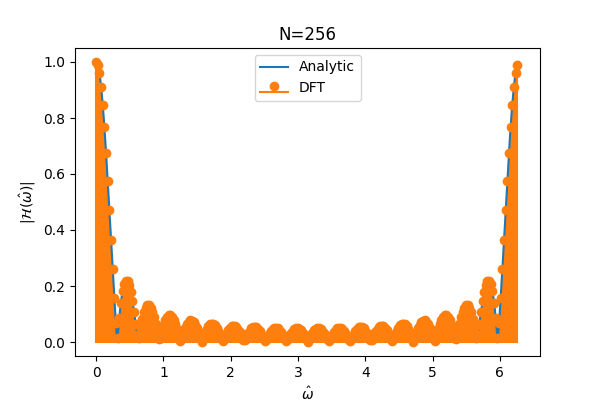
\includegraphics[width=1.5\textwidth]{code/020_dtft_estimate/dtft_estimate.png}
  \end{center}
  \caption{An estimate of the discrete-time Fourier transform evaluated using a DFT.}
  \label{fig:dtft_estimate}
\end{marginfigure}

\lstinputlisting[language=Python, caption={\texttt{020\_dtft\_estimate/dtft\_estimate.py}}, label=lst:dtft_estimate]{code/020_dtft_estimate/dtft_estimate.py}

\section{Fast Fourier Transform}

In practical applications, one should rarely naively follow Equation
\ref{eq:dft_eq_2} to implement a DFT operation, because it is not a
very efficient way to numerically evaluate this operation for $N$
frequencies. There exists a much faster algorithm to calculate this
operation called the \index{Fast Fourier Transform}{Fast Fourier
  Transform} (FFT), which is mathematically equivalent to Equation
\ref{eq:dft_eq_2}. The algorithm is fast, because it subdivides a long
Fourier transform into shorter discrete Fourier transforms in a
tree-like fashion.

\begin{marginfigure}
  \begin{center}
    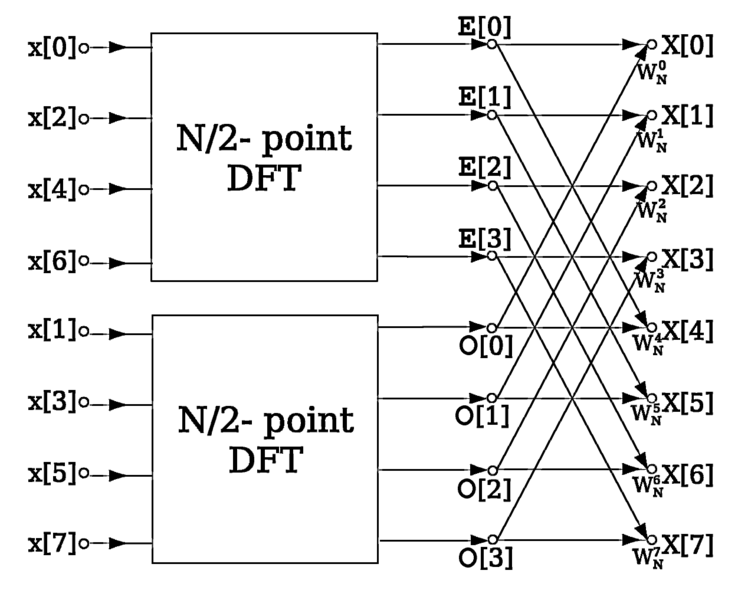
\includegraphics[width=\textwidth]{ch15/figures/butterfly.png}
  \end{center}
  \caption{The FFT speeds up the calculation by recursively subdividing an $N$ 
  length vector in half until the length of a vector has length 2. Credit: Virens (Wikimedia).}
\end{marginfigure}

The DFT as implemented using the mathematical formula (here $\phi_N
  = e^{-i\frac{2\pi}{N}}$):
\begin{equation}
  \hat{x}[k]=\sum_{n=0}^{N-1}x[n]\phi_N^{nk} \,\,,
  \label{eq:dft_eq_2}
\end{equation}
would require $\mathcal{O}(N^2)$ mathematical operations. The FFT
algorithm manages to perform mathematically the same operation by
using only $\mathcal{O}(N\log_2{N})$ operations\sidenote{This is big $\mathcal{O}$ notation from computer science,
  which is used to describe how the number of computations grows as a function of input size. $\mathcal{O}(N^2)$ means
  that when the input size grows by a factor of 10, the number of computations required will grow by a factor of 100.}.

The FFT algorithm makes use of the fact that you can divide a length
$N$ DFT into two length $N/2$ DFTs:
\begin{align}
  \hat{x}[k] & = \sum_{n=0}^{N-1}x[n]\phi_N^{nk}                                                                  \\
             & =\sum_{n=0}^{N/2-1} x[2n]\phi_{N/2}^{nk} + \phi_{N}\sum_{n=0}^{N/2-1} x[2n+1]\phi_{N/2}^{nk} \,\,.
\end{align}
A simple implementation of the first line takes $N^2$ operations, as
there are $N$ operations are needed for each of the $N$
frequencies. The second line is mathematically equivalent to the first
line, but it takes only $N^2/2$ operations, as there are two sums that
have $N/2$ unique frequencies and sum over $N/2$ terms ($2N^2/4 =
  N^2/2$ operations).

This subdivision of signals can be repeated until the length of each
DFT is 2. Each time the vectors are split in half, there is a
reduction by a factor of two in the number of operations that are
needed. A length $N$ signal can thus be split in half, approximately
$\log_2{N}$ times. Without going into further details, the end result
is a $N\log_2{N}$ computational complexity.%, where $\log_2{N}$ terms
%need to be added up for $N$ frequencies.

%, which
%means that the number of operations needed to compute a single
%frequency is proportional to $\log_2 N$. There are $N$ frequencies, so
%the resulting number of operations is proportional to $N\log_2
%N$. This is much faster than $N^2$ operations that are required, if
%the DFT formula is directly used.

\begin{marginfigure}
  \begin{center}
    
\includegraphics[width=\textwidth]{ch15/figures/fftwlogo.png}
  \end{center}
  \caption{The FFTW is included in many programming environments.
    In many situations, it is the fastest implementation of the FFT algorithm.}
\end{marginfigure}
Because the DFT is such a widely used and important algorithm, much
effort has been spent to optimizing it. Every scientific computing
environment includes one or more implementations of the FFT
algorithm. One of the most popular libraries is FFTW. In Python, the
PyFFTW module provides access to this library. There also exist GPU
optimized libraries, such as CuFFT, which allows NVidia graphics
acceleration cards to be used to calculate FFTs. In Python, one can
also use the \verb|numpy.fft| and \verb|scipy.fftpack| modules,
although neither of them is as efficient numerically as PyFFTW.


\section{Convolution}

%\lstinputlisting[language=Python,caption={\texttt{021\_fft\_convolution/fft\_convolution.py}},label=lst:fft_convolution]{code/signal_processing/021_fft_convolution/fft_convolution.py}

A \index{periodic convolution}{periodic convolution} is defined as:
\begin{equation}
  a[n] = \sum_{k=0}^{N-1} b[k]c[(n-k) \mod N] \,\,.
\end{equation}
In the case of DFT, multiplication in frequency domain is equivalent
to periodic convolution (denoted with symbol $\circledast$):
\begin{equation}
  \boxed{
    a[n] = b[n] \circledast c[n] \xleftrightarrow{\mathcal{F}_D} \hat{a}[k] = \hat{b}[k]\hat{c}[k]
  } \,\,.
\end{equation}

In order to implement a non-periodic convolution of two finite signals
of length $N$ and $M$, zero padding to length $N+M$ is needed. This
procedure is widely used to allow FFT to be used to compute a
convolution. The Scipy function \texttt{scipy.signal.fftconvolve} can
be used to convolve two signals using the FFT algorithm. It first
calculates $\hat{b}[k]$ and $\hat{c}[k]$, then multiplies them
together, and finally performs an inverse Fourier transform to obtain
the convolved signals.

\begin{marginfigure}
  \begin{center}
    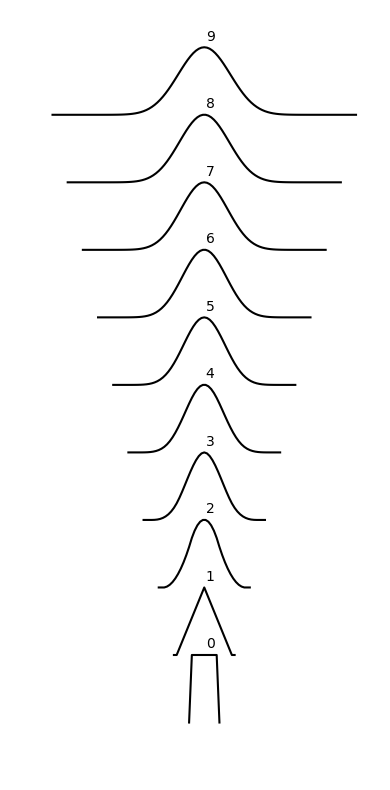
\includegraphics[width=\textwidth]{code/021_fft_convolution/central_limit.png}
  \end{center}
  \caption{Convolving a rectangular signal with itself over and over
    again will result in a Gaussian. See example: \texttt{021\_fft\_convolution/central\_limit.py}.}
  \label{fig:fft_convolution2}
\end{marginfigure}

\subsection{Example: Convolution using zero-padded FFT}

The Python code in Listing \ref{lst:fft_convolution} provides an
example of how to implement a convolution in frequency domain using a
zero-padded FFT. Because the FFT algorithm is so efficient
numerically, it is often advantageous to implement the convolution
operation using FFT. Figure \ref{fig:fft_convolution} shows the output
of the Python script.
\lstinputlisting[language=Python, caption={\texttt{021\_fft\_convolution/fft\_convolution.py}}, label=lst:fft_convolution]{code/021_fft_convolution/fft_convolution.py}


\section{Example: 2D FFT}

\begin{marginfigure}
  \begin{center}
    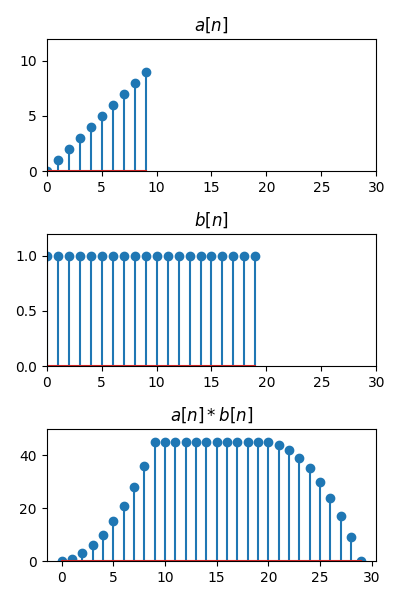
\includegraphics[width=\textwidth]{code/021_fft_convolution/convolution.png}
  \end{center}
  \caption{An example of a convolution of signals $a[n]$ and $b[n]$ evaluated using an FFT.}
  \label{fig:fft_convolution}
\end{marginfigure}


There also exists higher dimensional discrete Fourier transforms. For example, the 2D DFT is defined as:
\begin{equation}
  \hat{x}[k,\ell] = \sum_{n=0}^{N-1}\sum_{m=0}^{N-1} x[n,m] e^{-i \frac{2\pi}{N}nk }e^{-i \frac{2\pi}{N}m\ell } \,\,.
\end{equation}
There exists a 2D FFT algorithm that implements this efficiently, and
it is often used in image processing and image compression. There was
an example of the use of a 2D FFT for image compression in the Fourier
series chapter.

% ============ NOT USED ============
\if 0
  \subsection{Selected properties of DFT}

  Many of the familiar properties of the Fourier transform and the
  discrete-time Fourier transform also apply to discrete Fourier
  transforms. However, there are subtle differences. The main difference
  arises from periodicity of the time and frequency domain
  representation of signals.
  \begin{itemize}
    \item Periodicity $x[n+N]=x[n]$ and $\hat{x}[k]=\hat{x}[k+N]$.
    \item Linearity $\alpha_1 x_1[n] + \alpha_2x_2[n] \xleftrightarrow{\mathcal{F}_D} \alpha_1 \hat{x}_1[k] + \alpha_2 \hat{x}_2[k]$

    \item Spectral symmetry for real-valued signals. If $x[n] \in \mathbb{R}$, $\hat{x}[k]=\hat{x}^*[N-k]$. This also implies that $\hat{x}[0]\in \mathbb{R}$.

    \item Time symmetry for real-valued spectral representations. If $\hat{x}[k] \in \mathbb{R}$, $x[k]=x^*[N-k]$. This also implies that $x[0]\in \mathbb{R}$.

    \item Time shift is linear frequency dependent phase shift in frequency domain:\\ $x[n-n_0]\xleftrightarrow{\mathcal{F}_D} e^{-i\frac{2\pi}{N}k n_0}\hat{x}[k]$
    \item Linear time dependent phase shift in time domain is frequency shift in frequency domain:\\ $x[n]e^{i\frac{2\pi}{N}k_0 n} \xleftrightarrow{\mathcal{F}_D} \hat{x}[k-k_0]$
    \item Periodic convolution
          \begin{equation}
            a[n]=b[n]\circledast c[b]\xleftrightarrow{\mathcal{F}_D} \hat{a}[k]=\hat{b}[k]\hat{c}[k]
          \end{equation}
  \end{itemize}
\fi

% ============ END ============
